In this section we provide an overview of PaaS clouds and Cerebro. Then we present a model for 
negotiating response time SLAs for web APIs deployed in PaaS clouds.

\subsection{Properties of PaaS-hosted Applications}
PaaS clouds enforce a restricted programming model on the application developer to guarantee
the scalability, security and the availability of the cloud-hosted applications. To begin with,
PaaS clouds provide a predefined set of programming interfaces through which they export 
various platform services. We shall refer to these programming interfaces as the cloud software
development kit (cloud SDK). The cloud SDK exposes scalable functionality that can be used to 
program a wide range of application features. These include key-value data stores, databases, 
caching, task scheduling, and user management. In a typical PaaS environment
such as Google App Engine (or AppScale), the developer must use the cloud SDK to implement
all the required application components and APIs, as the use of third party services or libraries is
restricted within the cloud platform. 

Similarly, PaaS clouds may impose restrictions on performing
certain types of I/O operations, and executing long running tasks. For example, Google App Engine
denies applications access to the local file system (i.e. no file I/O). Furthermore, it forces the
developer to implement all application tasks as request-response interactions of a web service
where all requests must be processed
under 60 seconds. Any task that takes longer than this is terminated by the cloud platform.
This restriction is particularly interesting to us, since it gives a 60 second default SLA
for all web APIs developed for Google App Engine.
The result of all these restrictions is a programming model that is
amenable to reasoning via static analysis; a feature we exploit in the design of Cerebro. By surveying
a collection of open source PaaS applications we have also found that program features that typically
inhibit static analysis (e.g. excessive branching and loops) are scarce among PaaS-hosted
applications.

\subsection{Cerebro Architecture and Statistical Model}

\begin{figure}
\centering
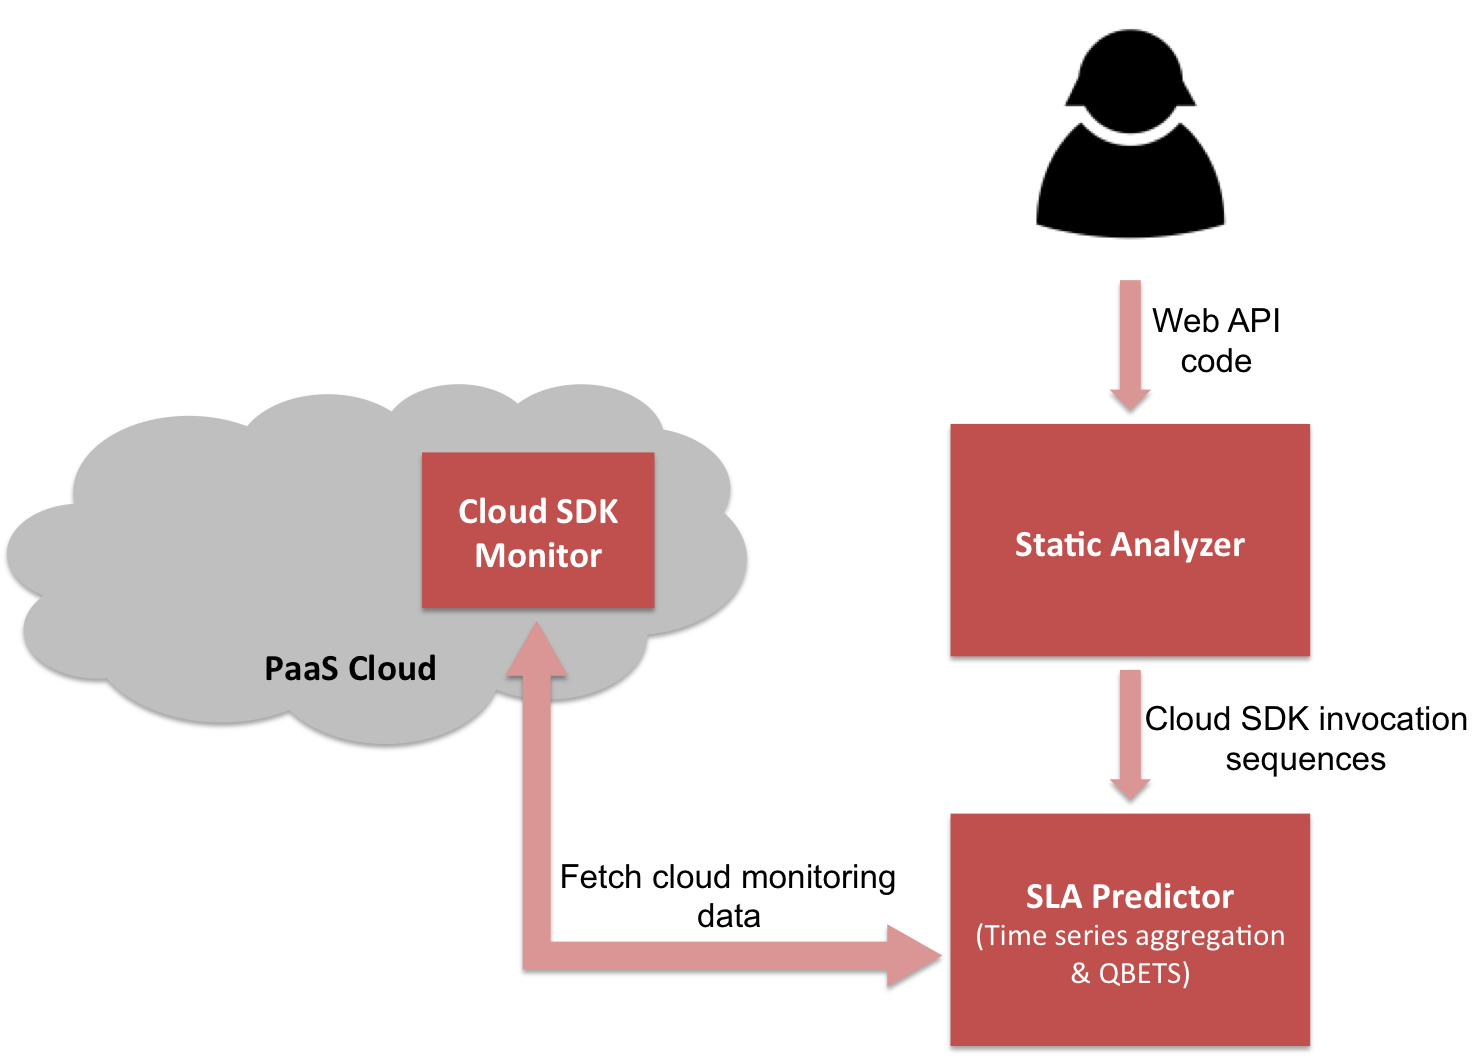
\includegraphics[scale=0.35]{cerebro_arch}
\caption{Main components of Cerebro and their interactions.}
\label{fig:cerebro_arch}
\vspace{-0.2in}
\end{figure}

Figure~\ref{fig:cerebro_arch} illustrates the main components of Cerebro, and how they interact with
each other. Cerebro runs a cloud SDK monitor in the PaaS cloud, that periodically benchmarks each
cloud SDK operation for execution time, and records the results as a set of time series (one time series 
per SDK operation). 
This component runs independent of all the applications deployed in the cloud, and it is active as long
as the cloud platform is available for serving requests. 

When an application developer submits a new
application to the cloud platform, Cerebro intercepts it, and runs it through a static analyzer.
Cerebro's static analyzer is designed to extract the sequence of cloud SDK operations invoked by each
web API operation in a given application. When the application code contains branches, it
extracts multiple sequences of cloud SDK operations -- one sequence per code path. The static
analyzer also looks for loops, and if any cloud SDK invocations are embedded within a loop, it attempts to
estimate loop bounds using existing loop bound analysis methods. If it fails, Cerebro prompts the 
application developer to provide a reasonable upper
bound for the loop count. Our survey results show that most of the time when loops are present in
a PaaS application, they simply iterate through a dataset loaded from the cloud datastore. 
Therefore, determining the bounds of such data-dependent loops is equivalent to establishing an 
upper bound for the size of the underlying datastore.

Having extracted the sequence of cloud SDK operations, Cerebro proceeds to invoke its SLA predictor.
The SLA predictor contacts the cloud SDK monitor to retrieve the gathered benchmarking data
pertaining to the cloud SDK operations used in the application. The predictor aggregates
this data according to the order and frequency of cloud SDK invocations in the application code, and forms a single
time series of benchmark results. This aggregate time series is then processed using QBETS (Queue
Bounds Estimation from Time Series), a 
non-parametric time series analysis and forecasting technique. QBETS analyzes the given time 
series, and predicts an upper bound for its $p$-th percentile, where $p$ is configurable. The predicted
value $Q$ can be used to form a response time SLA of the form ``the web API operation responds 
under $Q$ milliseconds at least $p$ percent of the time''.

The primary use of Cerebro is as a mechanism for predicting the response time SLAs for web APIs,
whenever a new web API is deployed to the cloud. However, our design also facilitates using
Cerebro as a development-time tool. That is, API developers can submit their work-in-progress
code to Cerebro in order to gain a preliminary set of SLA predictions. Further, we can use
Cerebro as a runtime tool, where it periodically re-evaluates the response time SLAs for 
APIs already deployed in the cloud.

Due to the dynamic nature of the cloud platforms, an SLA predicted on the cloud platform may not
hold correct forever. The performance of the individual cloud SDK operations vary over time, thus
affecting the response time of the web APIs deployed in the cloud. We use a
statistical model for detecting when a Cerebro-generated SLA becomes invalid. 
Suppose at time $t$ Cerebro predicts value $Q$ as the $p$-th percentile of
some API's execution time.  If $Q$ is a correct prediction,
the probability of API's next measured response time being greater than 
$Q$ is $1-(0.01p)$.  If the time series consists of independent
measurements then the probability of seeing $n$ consecutive values greater
than $Q$ (due to random chance) is $(1-0.01p)^n$. 
For example, using the $95^{th}$ percentile, the probability of seeing $3$
values in a row larger than the predicted percentile due to random chance
is $(0.05)^3 = 0.00012$.

This calculation is conservative with respect to autocorrelation. That is, if
the time series is stationary but autocorrelated, then the number of consecutive 
values above the $95^{th}$ percentile that correspond to a probability of
$0.00012$ is larger than $3$.  For example, in previous
work~\cite{Nurmi:2007:QQB:1791551.1791556}
using an artificially generated AR(1) series, 
we observed that $5$ consecutive values above the $95^{th}$ percentile
occurred with probability $0.00012$ when the first autocorrelation was $0.5$,
and $14$ when the first autocorrelation was $0.85$. QBETS uses a look-up
table of these values to determine the number of consecutive measurements above
$Q$ that constitute a ``rare event'' indicating a possible change in conditions.

Each time Cerebro makes a new prediction, it computes the current
autocorrelation and uses the QBETS rare-event look-up table to determine $C_{w}$:
the number of consecutive values that constitute a rare event.
We measure the time from when
Cerebro makes the prediction until we observe $C_{w}$ 
consecutive values above that prediction 
as being the time duration over which
the prediction is valid. We refer to this duration as the \textit{SLA validity duration}.  

In our prior work, we have implemented and tested a prototype of Cerebro on both Google 
App Engine public cloud, and the AppScale private cloud.
Our experiments have shown that Cerebro-generated SLA predictions are highly accurate. That is, when 
Cerebro predicts an SLA for some percentile $p$, the actual response time of the API (measured
independent of Cerebro) is less
than or equal to the predicted upper bound at least $p\%$ of the time. Further, we have shown that Cerebro
generates tight predictions. That is, predictions are sufficiently close to the actual response time
values. Finally, we have shown that Cerebro predictions stay valid for a sufficiently long period.  

\subsection{SLA Negotiation Model}